\documentclass[a4paper,titlepage,10pt,oneside]{article}

\usepackage[utf8]{inputenc} % Para poder escribir acentos directamente
\usepackage[spanish]{babel} % Para que el LaTeX sepa que el texto está en español y divida las sílabas al final de una línea correctamente, entre otras cosas
\usepackage[left=3cm, right=3cm, top=3cm, bottom=3cm]{geometry} % Para ajustar los márgenes, ya que por defecto son mayores
\usepackage{graphicx} % Para insertar imágenes
\usepackage[numbers]{natbib}
\usepackage[nottoc,notlot,notlof,numbib]{tocbibind}
\usepackage[font=scriptsize,format=plain,labelfont=bf,textfont=it,justification=centerlast]{caption}
\usepackage{listings}
\lstset{language=[ANSI]C, basicstyle=\scriptsize\ttfamily, keywordstyle=\color{Bittersweet}, commentstyle=\color{white}}
\lstset{numbers=left, numberstyle=\tiny, numbersep=5pt}

\usepackage{fancyhdr} % Para definir encabezados y pies de página personalizados
\pagestyle{fancy}
\fancyhead[L]{EUITI de Bilbao \\ Universidad del País Vasco} % Páginas pares e impares, alineado a la izquierda en la cabecera
\fancyhead[R]{Unai Martinez Corral \\ umartinez012@ikasle.ehu.es} % Páginas pares e impares, alineado a la derecha en la cabecera
\fancyfoot[C]{\thepage} % Páginas pares e impares, centrado en el pie
\fancyfoot[L]{Acher - Trabajo monográfico} % Páginas pares e impares, alineado a la izquierda en el pie
\fancyfoot[R]{2010-2011} % Páginas pares e impares, alineado a la derecha en el pie

\usepackage[usenames,dvipsnames]{color}
\usepackage[
    bookmarks=true,
    unicode=true,
    pdftitle={Acher},
    pdfsubject={Empleo del Ordenador Personal en la Instrumentacion de Panel},
    pdfauthor={Unai Martinez Corral},
    linktoc=all,
    colorlinks=true,
    linkcolor=Blue,
    urlcolor=BlueViolet,
    citecolor=Blue,
    ]{hyperref}

\renewcommand{\spanishtablename}{Tabla}
\renewcommand{\spanishlisttablename}{Índice de tablas}

\renewcommand{\footrulewidth}{0.4pt}
\renewcommand{\footnoterule}{\vspace*{15pt}
  \noindent\rule{1cm}{0.4pt}\vspace*{2.6pt}}

\parskip=2mm

%--------------------------------------------------------------------------

\title{
\begin{center}
 
\includegraphics[width=400pt]{./images/acher_logo.png}
\end{center}
\vspace{2.5cm}
\Huge{v0.1}
\vspace{1cm}
}

\author{
\LARGE{\textbf{Unai Martinez Corral}} \\
\\
\large{umartinez012@ikasle.ehu.es} \\
\vspace{1cm} \\
\large{\textbf{Empleo del Ordenador Personal en la Instrumentación de Panel}}\\
\\
\large{EUITI de Bilbao}
\vspace{2.25cm}
}

\date{\LARGE{2010-2011}}

%--------------------------------------------------------------------------

\begin{document}

\maketitle

%--------------------------------------------------------------------------

\tableofcontents

\newpage

\listoffigures

\listoftables

%--------------------------------------------------------------------------

\newpage
\section{Sobre Acher}

El objetivo de este proyecto es diseñar y construir un sistema para el control de carteles de texto formados por matrices de LEDs de forma dinámica y gestionar a través de un ordenador la información que en ellas se muestra. Lo que en un principio surgió como un reto personal, se ha enmarcado en el contexto de un trabajo monográfico para la asignatura \href{http://www.industria-ingeniaritza-tekniko-bilbao.ehu.es/p229-content/es/contenidos/informacion/euiti_bi_iti_electronica/es_oferta/adjuntos/19797.pdf}{Empleo del Ordenador Personal en la Instrumentación de Panel}, impartida en la \href{http://www.industria-ingeniaritza-tekniko-bilbao.ehu.es/}{Escuela Universitaria de Ingeniería Técnica Industrial de Bilbao}, centro perteneciente a la \href{http://ehu.es/}{Universidad del País Vasco / Euskal Herriko Unibertsitatea}.

El proyecto se ha estructurado en tres partes claramente diferenciadas: adquisición, transmisión y muestra de información. Todas ellas son en realidad independientes y podrían ser sustituidas por otras de idéntica funcionalidad, sin que el funcionamiento de las otras se viera afectado. Por ello, analizaremos cada una de las partes por separado, obviando la existencia del resto, aunque especificando las condiciones necesarias para que el proyecto funcione al unirlas. 

\subsection{Wishlist}

A continuación se listan aquellas funcionalidades que por falta de tiempo no se han implementado en esta revisión:

\begin{itemize}
  \item{Completar el contenido de CHAR\_ROM para la totalidad de los caracteres ASCII (ahora sólo están las mayúsculas y algunos caracteres sueltos).}
  \item{Diseñar uno o varios PCBs para la fabricación de un sistema real, y no sólo el prototipo.}
  \item{Diseñar e implementar la lógica necesaria para permitir la programación en circuito, evitando así la necesidad de un programador externo.}
  \item{Averiguar cómo trabajar con rutas y referencias relativas en LabVIEW (variables del tipo \$self o \$thispath).}
  \item{Ofrecer al usuario la opción de ver en la propia aplicación lo que debería mostrarse en la matriz de LEDs.}
  \item{Implementar órdenes mediante sentencias de escape para que el usuario pueda seleccionar diferentes formas de visualización en la matriz. Para lo cual también es necesario programar diferentes rutinas, a atender por la interrupción de columna, en el microcontrolador.}
  \item{Implementar órdenes mediante sentencias de escape para que el usuario pueda seleccionar la velocidad de desplazamiento del texto.}
  \item{Probar diferentes programas libres y multiplataforma, tanto para el desarrollo de la aplicación de usuario final como para el desarrollo y depurado del programa del microcontrolador.}
\end{itemize}
  
Se espera puedan ser añadidas en un futuro por el propio desarrollador o por terceras personas, en virtud de la licencia utilizada para la distribución del proyecto y del código fuente.

\subsection{Atribuciones y agradecimientos}

Para la programación del microcontrolador utilizado en el proyecto y para el diseño del circuito electrónico se ha utilizado como referencia el artículo \textit{Funcionamiento de una matriz de LEDS}\cite{ucontrol_leds} publicado por Ariel Palazzesi en la revista electrónica uControl.

\textit{LabVIEW}\cite{labview} es el nombre de un producto de la empresa \textit{National Instruments Corporation}\cite{ni}. Todas las figuras de la sección \hyperref[sec:adquisicion]{Adquisición} se han obtenido de \textit{LabVIEW} o de la ejecución de programas desarrollados con \textit{LabVIEW}.

El desarrollador quiere y debe agradecer el inestimable apoyo de Iñigo Oleagordia, profesor en la EUITI de Bilbao (UPV/EHU), al haber facilitado todos los recursos, tanto materiales como bibliográficos, solicitados.

Toda la documentación del programa (este documento), a excepción de aquellas figuras capturadas directamente de \textit{LabVIEW}, se ha creado y modificado con software libre. A continuación se citan los programas utilizados:

\begin{itemize}
  \item{LaTeX}
  \item{Gedit}
  \item{Notepad++}
  \item{Inkscape}
  \item{Dia}
  \item{Gimp}
  \item{Qucs}
  \item{KiCAD}
\end{itemize}
  
\subsection{Licencia}

\begin{center}
 
\includegraphics[width=200pt]{./images/ccby.png}
\end{center}

Este documento, a excepción hecha del código fuente, se distribuye bajo licencia Creative Commons By 3.0 (CC-by-3.0). Están permitidas la copia, distribución, y comunicación pública de la obra, así como su modificación y adaptación, siempre y cuando se reconozca la autoría mencionando a Unai Martínez Corral (pero no de una manera que sugiera que tiene su apoyo o apoya el uso que hace de su obra).

El \href{http://creativecommons.org/licenses/by/3.0/legalcode}{texto legal} completo está disponible en la página de la organización \href{http://creativecommons.org}{Creative Commons}:
\begin{center}http://creativecommons.org/licenses/by/3.0/legalcode\end{center}

\vspace{1cm}

\begin{center}
 
\includegraphics[width=100pt]{./images/gpl.png}
\end{center}

El código fuente del programa se distribuye bajo licencia GPL, tal como lo indican las cabeceras de los ficheros que lo contienen. En el fichero LICENSE.txt puede encontrarse el texto legal completo. También está disponible en la página del \href{http://www.gnu.org}{proyecto GNU}.


\newpage
\section{Adquisición}
\label{sec:adquisicion}

De las tres partes principales que componen el proyecto, ésta es la única en la que el desarrollador no ha tenido opción de decisión. Debido a su voluntad de presentarlo como trabajo monográfico para una asignatura, se ha visto en la obligación de adecuarlo para poder relacionarlo con ésta. Por ello, se ha optado por el desarrollo de la interfaz de usuario y la gestión del envío a través de \textit{LabVIEW}\cite{labview}, software desarrollado por \textit{National Instruments}\cite{ni} y centrado en la instrumentación electrónica.

Sin duda, y como podrá comprobarse a continuación, el consumo de recursos derivado de la adopción de esta solución resulta excesivo para la aplicación deseada. Si bien se trata de un software con gran utilidad en otros ámbitos, en éste en concreto y siempre bajo el punto de vista del autor, su uso podría definirse con la expresión ``matar moscas a cañonazos''. La extensa lista de herramientas, tanto gratuitas como libres y además multiplataforma, que podrían haberse utilizado resulta difícil de reproducir. Por poner algunos ejemplos, podrían mencionarse las bibliotecas GTK+\cite{gtk} y Qt\cite{qt}, en conjunto con cualquiera de los muchos lenguajes de programación que las soportan (C++, Java, Ruby, D, Perl, Python, PHP...). Como ya se expondrá en la sección \ref{sec:transmision}, correspondiente a la transmisión, la interfaz y protocolo utilizados están ampliamente extendidos y se dispone de librerías en prácticamente la totalidad de los lenguajes.

Tras esta introducción, se presenta la aplicación en sí, creada como un VI y posteriormente empaquetada en un ejecutable, que finalmente se ha utilizado para la generación de un instalador. Se perciben dos partes muy diferenciadas\footnote{El diagrama completo se encuentra en el \hyperref[anexoa]{Anexo A}} en ésta y así se presentarán: por un lado la aplicación base (aquella encargada de adquirir y enviar los datos) y por otra todos los aspectos estéticos que contribuyen a la apariencia del programa pero resultan inútiles desde un punto de vista operativo.

\subsection{Aplicación base}

La base de esta parte del proyecto es la adquisición de datos y el envío de éstos a través de la interfaz seleccionada. Como puede verse en la figura \ref{fig:acher_visa}, todo ello se consigue mediante tres bloques específicamente desarrollados para transmitir cadenas de caracteres a través del puerto de serie. El primero de ellos, obtenido con el nombre \textit{VISA Configure Serial Port} en el grupo \textit{VISA} dentro del apartado \textit{Instrument I/O} de la paleta de funciones, recibe los parámetros de configuración para definir el funcionamiento del protocolo, que más adelante se tratará en el apartado \ref{subsec:trama}.

\begin{figure}[!htp]
\centering
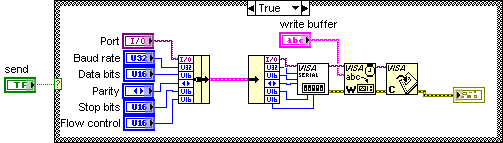
\includegraphics[width=300pt]{./images/acher_visa.png}
\caption{Envío de datos con \textit{LabVIEW}.}
\label{fig:acher_visa}
\end{figure}

Con el objetivo de hacer la aplicación lo más versátil posible, dentro de las limitaciones que su naturaleza establece, se han creado controladores para que el usuario tenga la posibilidad de configurar el tipo de comunicación, aunque están fijados por defecto los valores utilizados en este proyecto.

Para mejorar la legibilidad del código, se han unido todas las señales de los controladores en un cluster que después se ha separado a la entrada del bloque. En este caso en concreto, no supone una gran ventaja, pero es un avance de cara a futuras modificaciones.

El segundo bloque, \textit{VISA Write}, recibe como parámetro el string a enviar. Tal como se ha diseñado, envía los caracteres del string uno a uno, de forma secuencial y una sola vez. El bloque permite la especificación de un pequeño retardo entre caracteres. Se han realizado pruebas y se ha constatado que para la aplicación que se ha desarrollado no es necesaria la inclusión de dicha funcionalidad. El string a enviar se ha definido como un controlador, pues el objetivo es que el usuario final pueda decidir qué mostrar en la matriz de LEDs, y no que se envíe siempre el mismo contenido.

El último de los bloques, \textit{VISA Close}, cierra y termina la comunicación. La figura \ref{fig:acher_visa} muestra cómo se ha pasado el apuntador que indica el puerto a utilizar de un bloque a otro. Lo mismo se ha hecho con el cluster de error. Que finalmente enlaza con un \textit{Simple Error Handler}, para que el usuario pueda tener constancia e información cuando suceda algún error en la comunicación.

\subsection{Apariencia}

\subsubsection{Interfaz}

Una vez definida la funcionalidad base de la aplicación y para mejorar la apariencia de ésta, haciendo más fácil y visual su uso, se han realizado múltiples modificaciones mediante el uso de \textit{Property nodes} principalmente, aunque también se han utilizado otros recursos.

Se ha creado un indicador personalizado\cite{customcontrol} para mostrar una imagen en formato PNG con transparencia. Esta imagen corresponde al logotipo del proyecto que puede verse en la figura \ref{fig:acher_front}. No es ésta la forma más elegante de mostrar una imagen estática, pues para eso se dispone de otros recursos específicos, pero ha resultado la más fácil y rápida desde el punto de vista del desarrollador. Se ha modificado un indicador de tipo booleano para que muestre la misma imagen independientemente del valor que se le asigne. Este indicador puede encontrarse con el nombre \textit{logo\_acher.ctl} entre las fuentes del proyecto.

El controlador de tipo string que define el contenido a enviar por la aplicación se ha configurado mediante \textit{Property nodes} para que el texto aparezca siempre centrado y el tamaño sea mayor que el que aparece por defecto. Estos parámetros son constantes, por lo que el usuario no puede modificarlos durante la ejecución.

\begin{figure}[!htp]
\centering
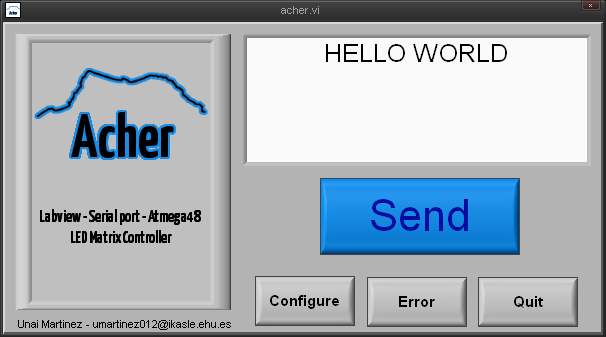
\includegraphics[width=300pt]{./images/acher_front.png}
\caption{Panel frontal: vista general.}
\label{fig:acher_front}
\end{figure}

Se han creado cuatro botones (controladores booleanos) para que el usuario pueda interactuar con la aplicación. Éstos son \textit{Send}, \textit{Configure}, \textit{Error} y \textit{Quit}.

\begin{itemize}

\item{\textbf{Send}:

La función de este botón es enviar, al pulsar sobre él, el contenido del controlador de tipo string:

Todo el programa se encuentra dentro de un bucle \textit{while}. El valor del botón \textit{Send} controla una estructura \textit{case} dentro del \textit{while}. Cuando es verdadera, se ejecuta la aplicación base analizada en la sección anterior. Mientras sea falsa, no se ejecuta acción ninguna.

Mediante los \textit{Property nodes} se han modificado el tamaño y color del texto y el color de fondo del botón. Este último, además, cambia cuando el botón está pulsado. El texto se encuentra en todo momento centrado tanto vertical como horizontalmente.
}

\item{\textbf{Configure}:

Este botón muestra y oculta los controladores que definen los parámetros a utilizar por el bloque \textit{VISA Configure Serial Port}. Para ello, actúa sobre la propiedad de visibilidad de éstos, además de sobre la misma propiedad del indicador utilizado para mostrar el logotipo y el \textit{Simple Error Handler}. También afecta al parámetro \textit{Disabled} del controlador string, del botón \textit{Send} y del botón \textit{Error}.

\begin{figure}[!htp]
\centering
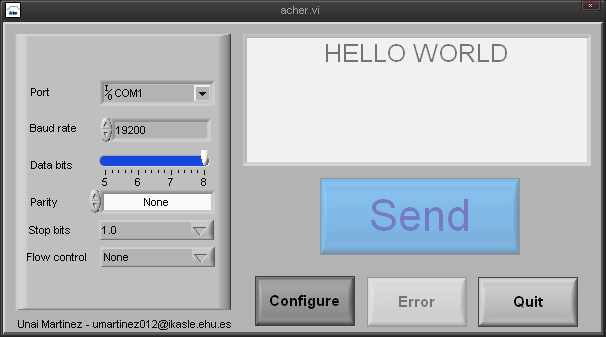
\includegraphics[width=275pt]{./images/acher_config.png}
\caption{Panel frontal: configure.}
\label{fig:acher_config}
\end{figure}

De esta manera, cuando el botón se encuentra pulsado y por lo tanto su valor es verdadero (Figura \ref{fig:acher_config}), se muestran únicamente los controladores de configuración, deshabilitando el controlador string y los botones \textit{Send} y \textit{Error}. El logo y el gestor de error se ocultan. Una vez el usuario ha realizado las modificaciones oportunas, la desactivación del botón \textit{Configure} devuelve la aplicación al estado mostrado en la vista general (Figura \ref{fig:acher_front}).

El tamaño del texto del botón y su alineación tanto horizontal como vertical se encuentran definidas mediante constantes.
}

\item{\textbf{Error}:

\begin{figure}[!htp]
\centering
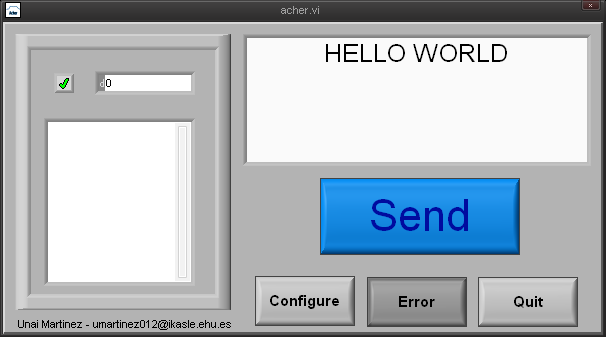
\includegraphics[width=275pt]{./images/acher_err1.png}
\caption{Panel frontal: no error.}
\label{fig:acher_err1}
\end{figure}

El funcionamiento de este botón, muy parecido al de \textit{Configure}, simplemente oculta el logo y muestra el gestor de errores cuando se encuentra pulsado (Figura \ref{fig:acher_err1}). Se debe tener en cuenta que \textit{Configure} tiene prioridad sobre \textit{Error}, por lo que el primero deberá estar desactivado para poder ver el gestor de errores.

El tamaño del texto del botón y su alineación tanto horizontal como vertical se encuentran definidas mediante constantes y mantienen su valor durante toda la ejecución. No así el color de fondo. Cuando se detecta algún error en el envío, éste cambia a rojo (Figura \ref{fig:acher_err2}), indicando así que no se ha efectuado correctamente.

\begin{figure}[!htp]
\centering
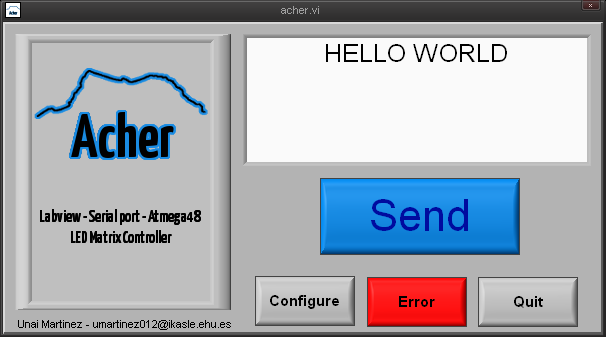
\includegraphics[width=275pt]{./images/acher_err2.png}
\caption{Panel frontal: error.}
\label{fig:acher_err2}
\end{figure}

Pulsando sobre el botón, se puede ver cuál es el error (Figura \ref{fig:acher_err3}). Para diferenciar cuándo se encuentra pulsado y cuándo no, en la nueva definición de color se han especificado dos constantes diferentes, siendo el segundo ligeramente más oscuro. Un simple \textit{select} controlado por el estado del botón booleando \textit{Error} decide cuál utilizar.

\begin{figure}[!htp]
\centering
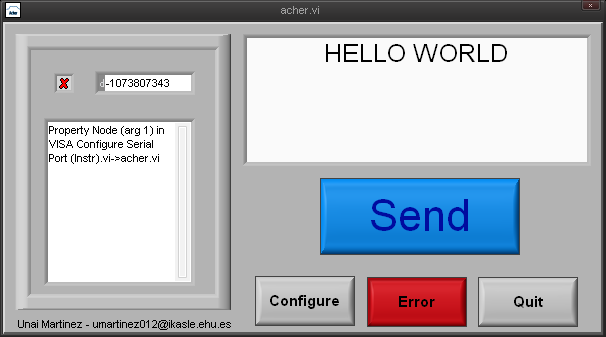
\includegraphics[width=275pt]{./images/acher_err3.png}
\caption{Panel frontal: view error.}
\label{fig:acher_err3}
\end{figure}
}

Al realizar un nuevo envío correcto, y por lo tanto no haber ningún error en el gestor de errores, el botón adquiere de nuevo el color original.

\item{\textbf{Quit}:

Para evitar que el usuario salga de la aplicación por error, la pulsación del botón \textit{Quit} controla una estructura \textit{case}. Cuando el valor es falso, éste se pasa directamente al controlador que termina el bucle \textit{while}, permitiendo que la aplicación siga ejecutándose. Cuando es verdadero, se lanza una ventana que pide confirmación al usuario (Figura \ref{fig:acher_quit}).

\begin{figure}[!htp]
\centering
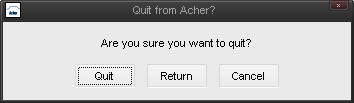
\includegraphics[width=175pt]{./images/acher_quit.png}
\caption{Ventana de salida.}
\label{fig:acher_quit}
\end{figure}

El lanzamiento de esta ventana se efectúa mediante el bloque \textit{Three Button Dialog}. Éste recibe como parámetros el contenido de los tres botones, el título de la ventana, el texto a mostrar y la alineación (Figura \ref{fig:acher_quitcase}). Un bloque de comparación hace que la salida sólo sea verdadera cuando el usuario pulse sobre el botón de la izquierda (\textit{Quit}). Cualquiera de las otras opciones (\textit{Return} o \textit{Cancel}), devolverá una salida falsa, permitiendo que se siga ejecutando el bucle principal.

\begin{figure}[!htp]
\centering
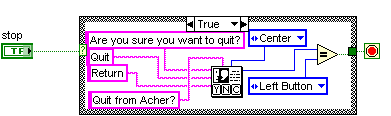
\includegraphics[width=225pt]{./images/acher_quitcase.png}
\caption{Lógica de salida.}
\label{fig:acher_quitcase}
\end{figure}
}

\end{itemize}

\subsubsection{Icono, patrón y ventana}

El icono y el patrón del VI se han personalizado para adecuarlos al proyecto. El icono reproduce el logotipo\footnote{El icono está disponible en las fuentes con el nombre \textit{acher\_icon.ico}}, mientas el patrón indica que no hay ninguna salida ni entrada, pues se trata de un VI que trabaja de forma autónoma.

Por otra parte, en las propiedades del VI se ha configurado como de tipo \textit{ventana de diálogo} para que no aparezcan los controles propios de \textit{LabVIEW} durante a ejecución. Además, el tamaño de ésta se ha adecuado al del panel frontal.

\subsection{Ejecutable e instalador}

Con el fin de facilitar el uso de la aplicación y para favorecer su portabilidad (entre equipos, no entre plataformas), se ha creado un ejecutable a partir del VI desarrollado. Para realizar este proceso, simplemente se ha creado un proyecto\footnote{El fichero del proyecto está disponible en las fuentes con el nombre \textit{acher.lvproj}} y, tras realizar las selecciones pertinentes (icono, nombres, rutas, etc.), se ha construido mediante el \textit{Application Builder} del propio \textit{LabVIEW}. Una vez obtenido el ejecutable, y haciendo uso de la misma herramienta\cite{installer}, se ha construido un instalador. En éste, además del ejecutable, el icono y otras opciones de personalización, se han añadido \textit{NI LabVIEW Run-Time Engine 2009} y \textit{NI-VISA Runtime 4.5}, un conjunto de librerías y drivers que permiten la instalación y ejecución del programa en aquellos equipos donde no esté instalado \textit{LabVIEW}.

El resultado final es un instalador de aproximadamente 150MB que nos garantiza la posibilidad de ejecutar el programa en cualquier equipo con un sistema operativo compatible y un puerto serie. Las condiciones de distribución y utilización se rigen por la licencia de \textit{LabVIEW}, pues es el software sobre el que corre la aplicación.

\subsubsection{Cierre del VI}

\begin{figure}[!htp]
\centering
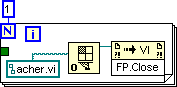
\includegraphics[width=150pt]{./images/acher_close.png}
\caption{Lógica de cierre del VI.}
\label{fig:acher_close}
\end{figure}

Debido a las características de ejecución de \textit{LabVIEW}, una vez terminado el bucle \textit{while}, es decir, cuando el usuario haya pulsado el botón \textit{Quit} y confirmado la acción en la ventana emergente, el VI se mantiene abierto, aunque parado. Aunque ésta es una característica muy útil (prácticamente imprescindible) en el proceso de desarrollo, resulta inadecuada en la aplicación final. Por un lado porque el usuario se ve obligado a cerrar una ventana más, a pesar de haber solicitado y confirmado el cierre de la aplicación. Por otro, porque una vez ha terminado la ejecución, e independientemente del tipo de configuración que se haya seleccionado en las propiedades del VI, se muestran menús propios de \textit{LabVIEW}. Éstos pueden producir confusión en el usuario, al desconocer su funcionalidad y la razón por la que aparecen. Además, en principio, no es de su interés el software utilizado para el desarrollo de la aplicación.

Para forzar el cierre del VI\cite{closevi} una vez se ha confirmado por parte del usuario, se ha añadido un bucle \textit{for} de una sola iteración (que actúa como un \textit{frame} secuencial) a continuación del \textit{while} principal (Figura \ref{fig:acher_close}). Dentro de éste encontramos un bloque del tipo \textit{Open VI Reference} al que se pasa como argumento el nombre del propio VI y un bloque \textit{Invoke Node} con el método \textit{Close FP} seleccionado que recibe el apuntador creado por el anterior.

\newpage
\section{Transmisión}
\label{sec:transmision}

Como interfaz de comunicación entre el ordenador personal y el microcontrolador encargado de controlar la matriz de LEDs, se ha optado por el puerto serie. La elección se ha basado en la sencillez y extensión de uso de éste. Dado que la velocidad de transmisión no resulta crítica en el sistema, no se ha considerado necesaria la implementación de otras interfaces más rápidas que conllevan el uso de conectores más grandes o de protocolos más complejos en su gestión.

Se trata de un puerto compatible con el estándar \textit{RS232} o \textit{EIA232 Standard}, cuyo uso con el conector DB-9 es un estándar de facto en las placas de desarrollo con microcontroladores, debido a que la gran mayoría de éstos integran periféricos específicos para la transmisión/recepción serie asíncrona.

Pese a que cada vez menos equipos de sobremesa incorporan puertos serie externos y que prácticamente ningún portátil los tiene, no es difícil encontrar adaptadores y extensores disponibles en el mercado. El autor considera que este contratiempo es un mal menor en comparación con las ventajas que esta interfaz ofrece.

\begin{table}[!htp]
\centering
\begin{tabular}[c]{|c|c|c|}
\hline
\multicolumn{2}{|c|}{\textbf{Señal}} & \textbf{DB-9} \\
\hline
Common Ground	    & G   & 5 \\ \hline
Transmitted Data    & TD  & 3 \\ \hline
Received Data	    & RD  & 2 \\ \hline
Data Terminal Ready & DTR & 4 \\ \hline
Data Set Ready	    & DSR & 6 \\ \hline
Request To Send	    & RTS & 7 \\ \hline
Clear To Send	    & CTS & 8 \\ \hline
Carrier Detect	    & DCD & 1 \\ \hline
Ring Indicator	    & RI  & 9 \\
\hline
\end{tabular}
\caption[Conexiones DB-9 según el estándar RS232]{Conexiones DB-9 según el estándar RS232, desde la perspectiva del DTE.}
\label{tab:db9}
\end{table}

De los nueve contactos que define el estándar para el conector (Tabla \ref{tab:db9}), sólo se han utilizado el contacto de masa común (5) y el de transmisión de datos (3), pues la comunicación será unidireccional. Si se quisiera que el microcontrolador enviara información al ordenador personal, se utilizaría también el contacto 2, recepción de datos.

\subsection{Interfaz física}
\label{subsec:trans_fis}

Las especificaciones de la norma en lo que a los niveles lógicos se refiere indican que la tensión para un cero lógico debe estar entre +3v y +15v; entre -3v y -15v para un uno lógico. De estos valores se deduce que los datos se transmiten con lógica negativa, al contrario que los microcontroladores habitualmente.

Por otra parte, los puertos de los microcontroladores no admiten ese rango de tensiones, pues están preparados para trabajar con señales TTL compatibles.

Por lo tanto, es necesario adecuar la tensión a valores TTL compatibles e invertir el valor lógico de los datos. Esto último podría omitirse si se implementara el protocolo a mano en el microcontrolador, o si el periférico dedicado a la comunicación serie de éste permitiera trabajar con lógica negativa. Para garantizar la compatibilidad con el mayor número de dispositivos posible, se obviará la omisión.

En el mercado se dispone de muchos circuitos que facilitan la conversión RS232-TTL y viceversa. Destaca especialmente el MAX232\cite{max232} de \textit{MAXIM}, que realiza las conversiones alimentándose únicamente de una fuente de +5v y utilizando cuatro condensadores externos para generar las tensiones necesarias.

Este chip pone a disposición del diseñador cuatro drivers, dos RS232-TTL y dos TTL-RS232. Aunque para este sistema en concreto sólo se ha utilizado un driver RS232-TTL, el uso de este integrado, y su correcto cableado, permitirá reutilizar el montaje para futura aplicaciones.

De acuerdo con las especificaciones disponibles en la hoja de características del circuito integrado, además de los cuatro condensadores para generar las tensiones RS232 compatibles, se ha necesitado un quinto para estabilizar la alimentación. Teniendo en cuenta la aplicación que se está tratando, todos ellos tienen una capacidad de 1$\mu$F.

\subsubsection{Esquema electrónico}

Asumiendo que sólo se ha utilizado uno de los drivers, no se ha prestado atención a los contactos asociados a los otros tres, pues su funcionamiento no afecta al sistema. El resto de contactos se han cableado según las indicaciones de la hoja de características, tal como ilustra la figura \ref{fig:esq_max232}.

\begin{figure}[!htp]
\centering
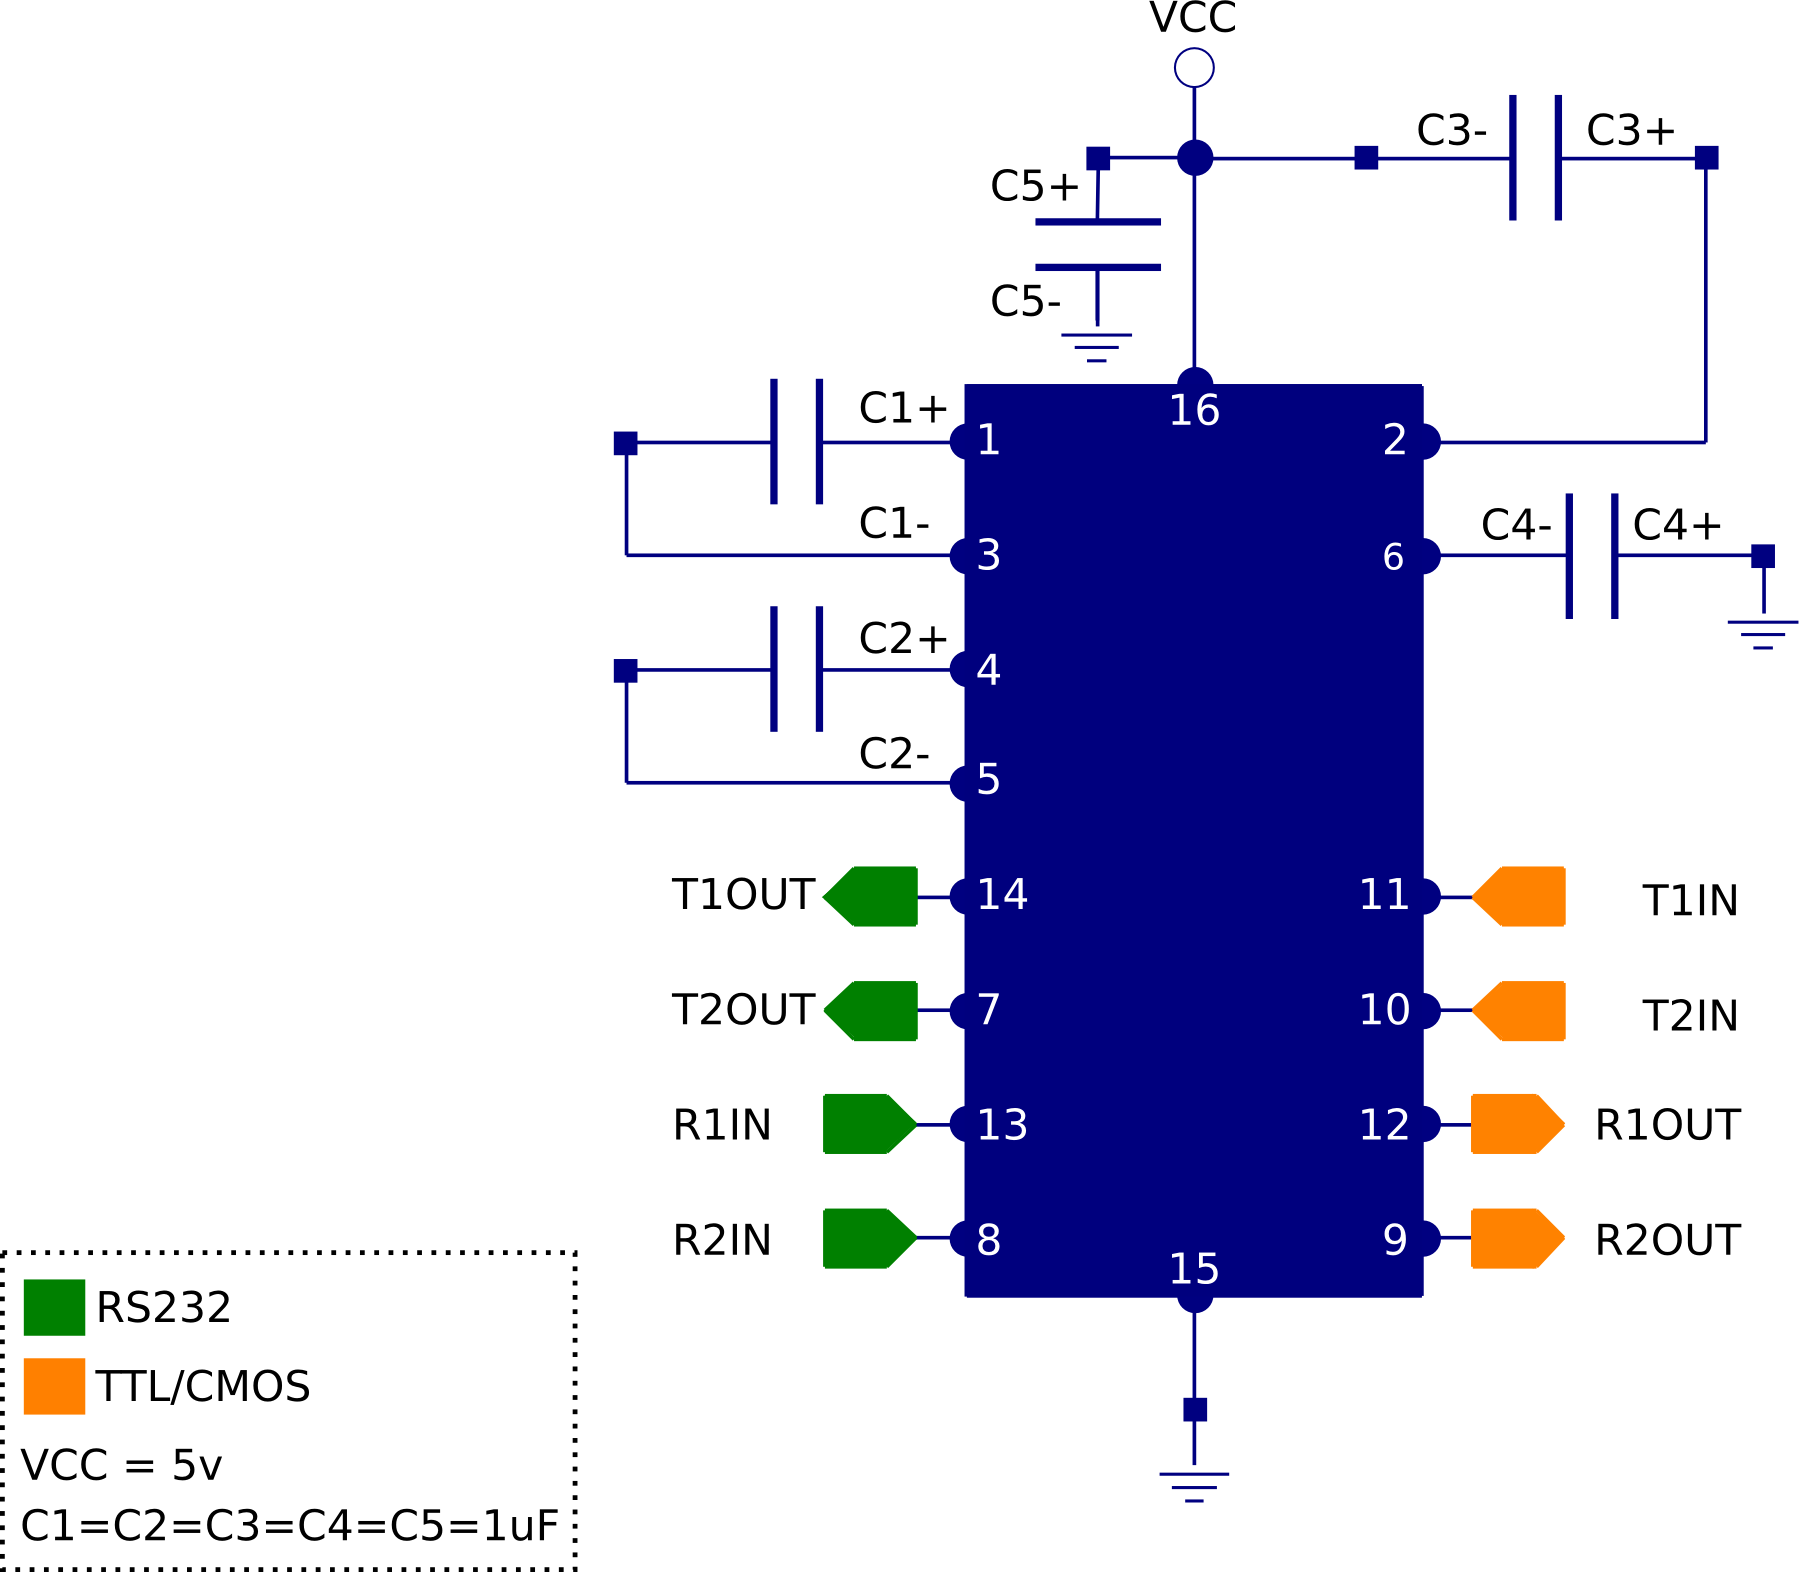
\includegraphics[width=300pt]{./images/esq_max232.png}
\caption{Esquema de conexionado del circuito integrado MAX232.}
\label{fig:esq_max232}
\end{figure}

\subsection{Formato de la trama}
\label{subsec:trama}

La norma RS232 comprende varios protocolos de entre los cuales cabe destacar la diferenciación entre \textit{síncronos} y \textit{asíncronos}. Los primeros requieren el uso de una señal de reloj que, gestionada por el maestro en la comunicación, sirve para sincronizar el envío de datos entre los componentes. En el caso de los asíncronos la transmisión se basa en el determinación de la temporización a ambos lados, de forma que se puede utilizar una sola línea modificando los datos con una frecuencia acordada.  Debido a que el número de conectores suele ser un bien preciado en los microcontroladores, se ha optado por utilizar una comunicación asíncrona, reduciendo de tres a dos el número de contactos necesarios para una comunicación unidireccional.

Atendiendo al protocolo establecido por la norma RS232 para las comunicaciones asíncronas sin tiempo de inicio preestablecido, la información se envía, como ilustra la figura \ref{fig:trama_rs232}, estructurada en cuatro partes:

\begin{itemize}
	\item{START: bit de inicio o arranque. Inicia la comunicación cuando la línea, que en estado de reposo se encuentra en un uno lógico, pasa a un cero lógico. A partir de este flanco, el receptor comienza a leer las señales con una frecuencia preestablecida.}
	\item{DATA: bits de datos. Se envía el número de bits preestablecido, empezando por el de menor peso, LSB (\textit{Least Significant Bit}), y terminando por el de mayor peso, MSB (\textit{Most Significant Bit}).}
	\item{PARITY: bit de paridad. Si se ha preestablecido la transmisión de un bit de paridad para comprobar la integridad de los datos, se enviará un uno o un cero lógico en función del tipo de paridad (par o impar) y la palabra enviada.}
	\item{STOP: bit de parada. La línea se mantiene en un uno lógico cuando termina la transmisión. Este bit, que puede mantenerse el equivalente a 1, 1.5 o 2 bits, indica la finalización de la transmisión.}
\end{itemize}

\begin{figure}[!htp]
\centering
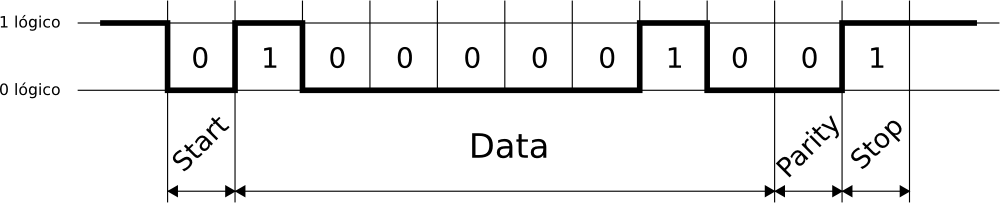
\includegraphics[width=300pt]{./images/trama_rs232.png}
\caption[Ejemplo de envío de una trama según RS232]{Ejemplo de envío de una trama según RS232. Código ASCCI de ``A'' (01000001), 8 bits de dato con paridad par y 1 bit de stop.}
\label{fig:trama_rs232}
\end{figure}

Dado que los datos a transmitir serán de tipo char y la integridad de los datos no resulta crítica, en este proyecto se ha optado por implementar una comunicación con un bit de start, ocho bits de dato, ninguno de paridad y un bit de stop. Éstos serán los datos a tener en cuenta por la aplicación que transmita los datos desde el ordenador, y la configuración del receptor del microcontrolador.

\subsection{Velocidad de transmisión}

La unidad más utilizada para expresar la velocidad de transmisión, la cantidad de información enviada, es el \textit{baudio} \cite{baudio}. Proporcional a los bits por segundo (bps), expresa el número de bits de información. La velocidad a la que pueden trabajar tanto los puertos serie de un ordenador como los microcontroladores está normalizada a 75, 150, 300, 600, 1200, 2400, 4800, 9600 baudios, etc.\cite{pic_serie}.

Para la aplicación que nos ocupa, se ha escogido una velocidad de transmisión de 19200 baudios. Si bien podrían utilizarse velocidades mayores, nuestro sistema no requiere una alta velocidad de transmisión y este valor facilita los cálculos para la configuración del microcontrolador, como se analizará en la sección correspondiente.


\newpage
\section{Muestra}

Para la gestión de la matriz de LEDs se ha optado por la utilización de un sistema basado en un microcontrolador, junto con diversos drivers que faciliten la programación y la adecuación de las señales. Aunque podría haberse gestionado toda la lógica desde el ordenador, esto habría vuelto el sistema directamente dependiente de éste, lo cual impediría su funcionamiento cuando estuviera apagado. La externalización de la lógica nos permite utilizar el ordenador únicamente para enviar el contenido a mostrar en la matriz, obteniendo un sistema autónomo una vez recibida la información. Si quisiéramos mostrar información preprogramada, en lugar de definir el contenido dinámicamente, el microcontrolador nos da la opción de cargar la información durante el diseño.

Asimilando las ventajas de implementar la lógica de forma externa al ordenador, el microcontrolador se muestra como una de las opciones, entre las cuales también debemos valorar el uso de FPGAs, CPLDs o VLSIs. El diseño con VLSIs y CPLDs resulta excesivamente complejo, debido a la necesidad de efectuar operaciones aritméticas de cierta complejidad y el uso de diversos registros. El diseño se complicaría lo suficiente como para no resultar rentable por el tamaño final del circuito y el número de integrados necesarios. Las FPGAs suplen a la perfección estas necesidades, pero su alimentación resulta más compleja que la de un microcontrolador, y el hecho de disponer de memoria volátil complica la implementación física, al ser necesaria la adición de elementos de memoria para evitar tener que programarlas en cada arranque. Además, ninguna de las opciones anteriores incorpora periféricos específicos para la temporización o la comunicación serie. Estos recursos deberían ser desarrollados por el diseñador. Por estas razones, un sistema microcontrolador se muestra como la mejor opción, al aunar la simplicidad de diseño del circuito y la complejidad de recursos necesaria para esta aplicación.

De entre los muchos microcontroladores disponibles en el mercado, se ha utilizado el modelo Atmega48 de Atmel\cite{atmega48}, con arquitectura AVR\cite{avr}. La elección de este modelo responde a la facilidad de acceso a los recursos para trabajar con él, pues el desarrollador ha tenido a su disposición un kit de desarrollo STK500\cite{stk500} del mismo fabricante. El modelo citado dispone de recursos suficientes para el sistema a desarrollar y permite la evolución de este de cara a añadir funcionalidades en futuras versiones. Además, la arquitectura AVR se diseñó específicamente para la ejecución eficiente de código C compilado, lenguaje utilizado por el desarrollador.

En cualquier caso, y dado que no se hace uso de recursos sólo disponibles en la arquitectura AVR, con la debida adecuación del código podría utilizarse cualquier otro microcontrolador para el cual se disponga de un compilador de C, ya sean los muy extendidos PIC\cite{pic} de Microchip, aquellos compatibles con el 8051\cite{8051} de Intel, u otros muchos disponibles en el mercado.

\subsection{Elección de componentes y esquema electrónico}

Antes de abordar la elección de componentes para el circuito, se ha efectuado una división basada en la funcionalidad de éstos\footnote{El esquema electrónico completo se encuentra en el \hyperref[anexob]{Anexo B}}. A saber:

\begin{itemize}
  \item{Circuito base: agrupa los componentes básicos para el funcionamiento del sistema basado en un microcontrolador, independientemente de su uso}
  \item{Recepción: agrupa los componentes necesarios para la recepción de la información según el estándar RS232, cuyo uso se ha justificado en la sección \ref{sec:transmision}.}
  \item{Muestra: agrupa los componentes necesarios para mostrar la información.}
\end{itemize}

\subsubsection{Circuito base}

Como resulta evidente, el componente principal necesario es el microcontrolador. De entre los muchos empaquetados disponibles\cite{atmega48}, se ha escogido el PDIP de 28 contactos. Esta elección se justifica por la facilidad de montaje. Debido a la naturaleza didáctica de este proyecto y puesto que es la primera vez que el autor utiliza muchos de los recursos, este empaquetado facilita el montaje de pequeños circuitos de prueba, el cambio de dichos circuitos al kit de desarrollo y viceversa, etc.

Para el correcto funcionamiento en esta aplicación en concreto, basta con alimentar el dispositivo con una tensión de aproximadamente 5v. Para ello, conectaremos una fuente al contacto 7 (Vcc) y la masa a los contactos 8 y 22 (GND). También deberemos conectar el contacto 20 (AVCC) a la tensión de alimentación, pues a pesar de no utilizar el conversor A/D, resulta necesario para un funcionamiento adecuado del circuito.

El modelo utilizado dispone de un oscilador RC interno que genera la señal de reloj (de hasta 8Mhz) necesaria para el funcionamiento del dispositivo. Aunque éste podría ser suficiente para muchas aplicaciones, la precisión no es todo lo buena que desearíamos para garantizar una comunicación serie fiable. Al tratarse de una comunicación asíncrona, las temporización cobra una importancia vital y por lo tanto deberemos disponer de una señal de reloj más estable.

Debido a que el microcontrolador dispone de los componentes y los contactos\cite{atmega48} (9:XTAL1 y 10:XTAL2) necesarios para amplificar y utilizarlo, y puesto que su uso está muy extendido, emplearemos un cristal oscilador externo. La frecuencia de éste, 11,0592 MHz, se ha escogido teniendo en cuenta los criterios de programación para la comunicación serie asíncrona. Pueden consultarse los detalles en la sección \ref{subsec:programacion}.

El uso de un oscilador externo de cristal exige la utilización de dos condensadores cerámicos de idéntica capacidad, tal como puede verse en la figura \ref{fig:esq_osc}. El valor de éstos, atendiendo a la información contenida en la hoja de características del microcontrolador\cite{atmega48}, se ha definido como 22pF.

\begin{figure}[!htp]
\centering
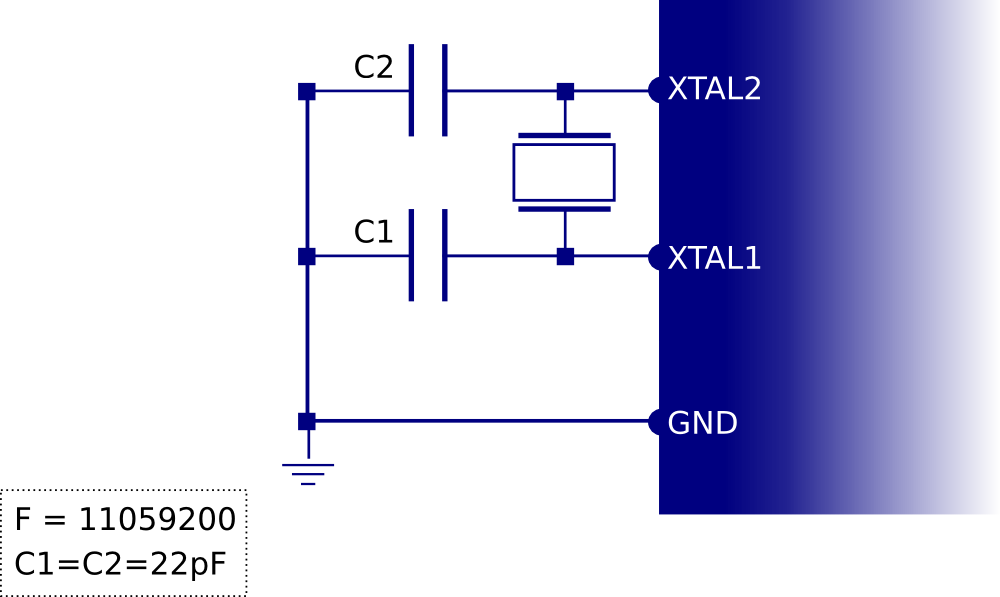
\includegraphics[width=300pt]{./images/esq_osc.png}
\caption{Esquema de conexión del oscilador externo.}
\label{fig:esq_osc}
\end{figure}

\subsubsection{Recepción}

Como el microcontrolador dispone de un periférico específico para la implementación de comunicaciones serie que permite el modo de trabajo asíncrono con dos contactos asociados en el empaquetado, siempre y cuando la señales sean TTL compatibles, no es necesaria la adición de ningún componente externo.

Tal como se ha descrito en la sección \ref{subsec:trans_fis}, las señales provenientes del ordenador se adecuan mediante el circuito integrado MAX232\cite{max232} a niveles apropiados. Simplemente se debe conectar la salida adecuada (en este caso R2OUT, el contacto 9 del integrado) a la entrada asociada en el microcontrolador, el contacto 2 (RXD).

\subsubsection{Muestra}
\label{subsubsec:muestra}

Una matriz de LEDs no es más que una serie de LEDs dispuestos de forma matricial y garantizando que todos aquellos situados en una fila tengan un contacto en común (en el diseño desarrollado, el ánodo), y aquellos situados en una columna el otro (el cátodo). La diferencia de tensión adecuada entre el ánodo (número de fila) y el cátodo (número de columna), encenderá el LED apropiado. Gestionando la tensión en todas las filas y todas las columnas se puede controlar qué LEDs se encienden y cuáles se mantienen apagados.

\begin{figure}[!htp]
\centering
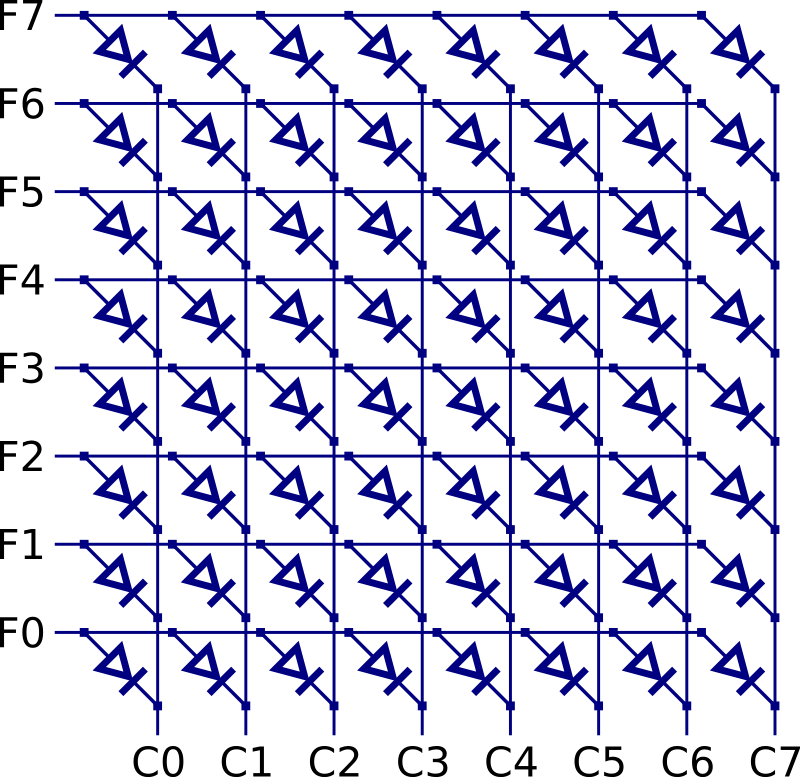
\includegraphics[width=200pt]{./images/esq_matriz.png}
\caption{Esquema de conexión de una matriz de LEDs 8x8.}
\label{fig:esq_matriz}
\end{figure}

La matriz puede fabricarse mediante la correcta colocación y conexionado de LEDs discretos, tal como ilustra la figura \ref{fig:esq_matriz}. Sin embargo, el número de contactos a conectar resulta lo bastante elevado como para resultar una labor tediosa: para una matriz de 8x8 se deben conectar 8x8x2=128 contactos. Existen en el mercado matrices ya empaquetadas con sólo el número de contactos correspondiente al número de filas y el número de columnas. Para una matriz de 8x8 se tendrían 8+8=16 contactos. La comodidad y el ahorro tanto en complejidad como en tiempo sin duda obligan a valorar muy positivamente esta posibilidad.

Para el desarrollo del prototipo de este proyecto, se ha utilizado un modelo comercial de 8x8\cite{matrix} del tipo columna-ánodo/fila-cátodo, debido a que era el modelo más accesible. Sin embargo, dado que la lógica se había considerado para una arquitectura donde las filas estuvieran conectadas a los ánodos, se ha optado por conectar los contactos descritos en la hoja de características como de columna a las filas, y viceversa.

La solución más rápida para gestionar una matriz de 8x8 mediante el microcontrolador consistiría en conectar cada uno de los contactos de ésta a un contacto del microcontrolador. Esto no resulta un problema para una matriz del tamaño descrito, pues disponemos de más 16 de contactos en el microcontrolador. Sin embargo, el objetivo de este proyecto es poder escalar el número de columnas para poder controlar carteles del tamaño deseado. Si se quisieran controlar 30 columnas, serían necesarios 38 contactos, de los cuales no se dispone. Es por esta razón por la que se ha optado por controlar la matriz de forma dinámica, haciendo uso de la multiplexación de las filas y utilizando registros de desplazamiento\cite{shiftr}.

Aprovechando que el microcontrolador funciona a una velocidad mucho mayor que la que el ojo humano es capaz de apreciar, se activarán las filas una por una, en lugar de encender todas ellas al mismo tiempo. Suponiendo que se trabaja con ocho filas, cada una de ellas estará encendida 1/8 parte del ciclo total de actualización. Como el ciclo total será menor que el tiempo mínimo apreciable, la sensación será la de estar viendo todas las filas iluminadas al mismo tiempo. Asumiendo que cada fila se encenderá por separado y nunca habrá dos de ellas activas al mismo tiempo, los LEDs que se encenderán vendrán determinados por el valor que tengan los contactos de las columnas en el momento de activación de una fila concreta. Ahí es donde cumplen su función los registros de desplazamiento: almacenarán los datos de las columnas durante el tiempo en que ésta esté activa. La comunicación entre el microcontrolador y un registro de desplazamiento es serie síncrona. Como es unidireccional, sólo necesitamos dos contactos, el de dato y el de reloj (que serán controlados por el microcontrolador), además de la masa.

De entre los registros de desplazamiento disponibles en el mercado, se ha optado por el 74HC164 \cite{164} en empaquetado PDIP de 14 contactos. Se trata de un modelo con dos contactos de entrada serie (1:A y 2:B), a las cuales se les realiza una operación lógica AND, y salida en paralelo de ocho bits. Puesto que no se necesitan las dos líneas de datos, se han conectado ambas entradas entre sí y al contacto de salida que se ha escogido en el microcontrolador para esta función (15:PB1). Las ocho salidas se han conectado a las respectivas columnas por medio de sendas resistencias \footnote{La función de las resistencias es limitar la tensión que caerá en los LEDs. El valor de éstas dependerá de la fuente con que se alimenten, como se verá al analizar la conexión de las filas.}, tal como describe la tabla \ref{tab:reg_col}.

\begin{table}[!htp]
\centering
\begin{tabular}[c]{|c|c|c|}
\hline
\multicolumn{2}{|c|}{\textbf{47HC164}} & \textbf{Matriz} \\
\hline
Q0 & 3 & C0 \\ \hline
Q1 & 4 & C1 \\ \hline
Q2 & 5 & C2 \\ \hline
Q3 & 6 & C3 \\ \hline
Q4 & 10 & C4 \\ \hline
Q5 & 11 & C5 \\ \hline
Q6 & 12 & C6 \\ \hline
Q7 & 13 & C7 \\
\hline
\end{tabular}
\caption{Conexiones entre el registro de desplazamiento y la matriz de LEDs.}
\label{tab:reg_col}
\end{table}

Los contactos de alimentación (14:VCC y 7:GND) se han conectado directamente a la fuente de alimentación. El reset global (9:$\overline{MR}$) se ha deshabilitado permanentemente dejándolo conectado a Vcc (el borrado se realizará por software al ejecutar la rutina de inicialización). El último contacto disponible, el de la señal de reloj (8:CP) se ha conectado al contacto escogido en el microcontrolador para dicha función (16:PB2).

Las salidas del microcontrolador pueden dar corriente suficiente para alimentar un reducido número de LEDs. Sin embargo, resulta claramente insuficiente a lo hora de trabajar con carteles de treinta, cuarenta o cincuenta columnas. En estos casos se debe utilizar un driver intermedio que actúe como etapa de potencia. Aunque el cartel del prototipo tiene pocas columnas, y a pesar de que en esas condiciones el microcontrolador podría alimentar los LEDs directamente, siempre es recomendable poner un driver para proteger el integrado de posible errores de montaje.

\begin{table}[!htp]
\centering
\begin{tabular}[c]{|c|c|c|}
\hline
\multicolumn{2}{|c|}{\textbf{Atmega48}} & \textbf{Matriz} \\
\hline
PC0 & 23 & F0 \\ \hline
PC1 & 24 & F1 \\ \hline
PC2 & 25 & F2 \\ \hline
PC3 & 26 & F3 \\ \hline
PC4 & 27 & F4 \\ \hline
PC5 & 28 & F5 \\ \hline
PD2 & 4  & F6 \\ \hline
PD3 & 5  & F7 \\
\hline
\end{tabular}
\caption{Conexiones entre el microcontrolador y la matriz de LEDs.}
\label{tab:filas}
\end{table}

En este proyecto las salidas del microcontrolador que deberán llevar driver son aquellas conectadas a las filas de la matriz de LEDs. Para conseguir la ganancia de potencia, se han utilizado transistores bipolares PNP\cite{140} que soportan una corriente de emisor de hasta 1.5A, lo cual permite conectar entre 75 y 100 columnas (en función de la corriente que consuman los LEDs). Al ser de tipo PNP, los transistores conducirán cuando la tensión en su base sea cero. Se debe tener en cuenta este hecho a la hora de realizar la programación de las rutinas del microcontrolador. Para desactivar una fila, por lo tanto, debería haber una tensión positiva en la base, lo cual se conseguirá activando la salida adecuada. Como sólo hace falta una pequeña corriente, se ha puesto una resistencia de 1K5 entre la salida y la base. El emisor de todos los transistores está conectado a la tensión de alimentación, mientras los colectores se conectan a las filas correspondientes de la matriz, de acuerdo con lo establecido por la tabla \ref{tab:filas}.

\begin{figure}[!htp]
\centering
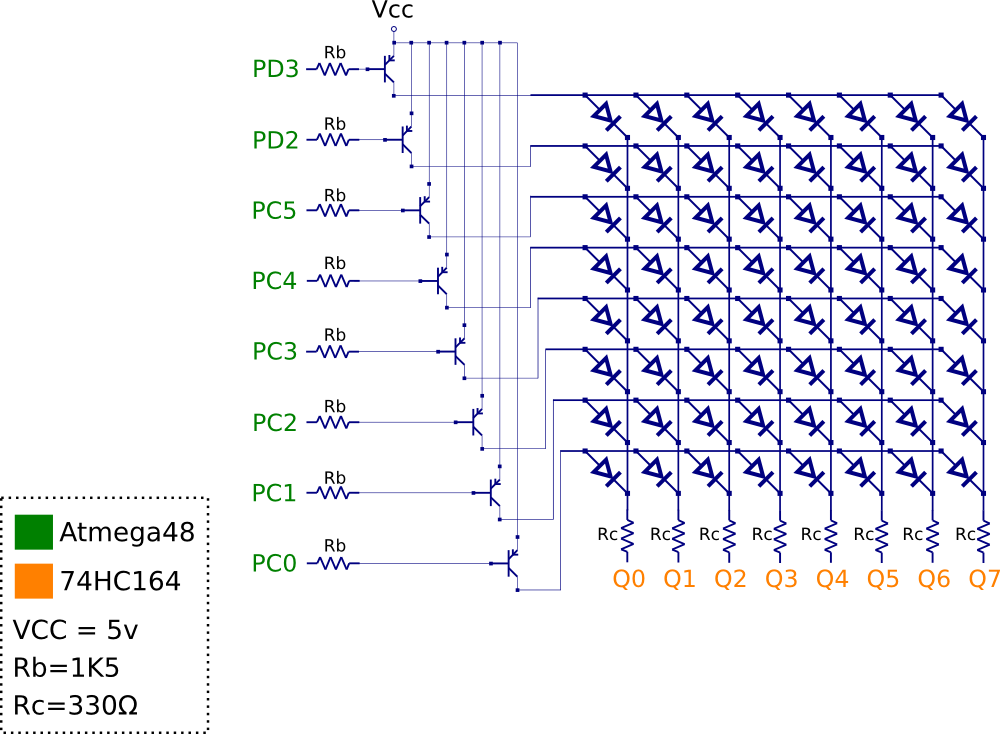
\includegraphics[width=350pt]{./images/esq_pnp.png}
\caption[Esquema de conexión matriz, microcontrolador y registro]{Esquema de conexión de la matriz al microcontrolador y al registro de desplazamiento.}
\label{fig:esq_pnp}
\end{figure}

Con la arquitectura descrita, cuando un transistor determinado conduzca y al menos una de las salidas del registro de desplazamiento esté a nivel bajo, habrá un LED que encuentre cero voltios (masa) en su cátodo y la tensión de alimentación en su ánodo. Lo más probable es que en estas condiciones el LED se queme, pues la alimentación será de aproximadamente cinco voltios. Para evitar que esto suceda, se podría sustituir la tensión en los emisores por una menor. Esto requiere dimensionar un divisor/reductor de tensión para soportar la corriente de todos los transistores. Desde un punto de vista práctico, resulta más fácil mantener ese mismo valor da alimentación e introducir resistencias entre los cátodos y las salidas del registro de desplazamiento, tal como ilustra la figura \ref{fig:esq_pnp}. Para el prototipo se han utilizado resistencias de 330$\Omega$.

\subsection{Programación}
\label{subsec:programacion}

Al ser el juego de instrucciones de la familia AVR desconocido para el desarrollador y no haber tenido nunca contacto con este tipo de microcontroladores, decidió para un primer acercamiento programar utilizando el lenguaje C, más concretamente el estándar ANSI. La arquitectura AVR está soportada por el compilador libre GCC\cite{gcc} y existe una implementación, también software libre, que permite utilizarlo bajo sistemas Windows, distribuida como WinAVR\cite{winavr} y que incluye compilador, programador y debugger.

Pese a la existencia de herramientas libres y multiplataforma para efectuar el desarrollo completo, se ha utilizado el AVR Studio 4\cite{avrstudio} como IDE. La elección de esta herramienta se justifica sólo por la seguridad de saber que se están utilizando recursos del propio fabricante que garantizan una alta compatibilidad con el kit de desarrollo. En cualquier caso, el uso de las herramientas de depurado y programación se escapan al objetivo de este documento, por lo que no se profundizará en su uso.

\subsubsection{Notas del desarrollador}

Si bien no son necesarias para la utilización del sistema, el desarrollador considera que las siguientes anotaciones pueden resultar de interés para quién quiera entender el desarrollo completo y qué decisiones se han tomado durante el mismo.

\begin{itemize}
  \item{\textbf{Estructura de ficheros}: la programación del microcontrolador se ha dividido en tres ficheros\footnote{El diagrama de flujo del programa completo se encuentra en el \hyperref[anexoc]{Anexo C}}:
    \begin{itemize}
      \item{\textbf{acher\_main.c}: contiene la función \textit{main} y las rutinas de vectorización de las interrupciones.}
      \item{\textbf{acher\_config.c}: contiene las rutinas de inicialización de variables y configuración de puertos y periféricos.}
      \item{\textbf{acher\_main.h}: contiene la declaración de constantes, variables y prototipos de las funciones.}
    \end{itemize}}
  \item{\textbf{Mayúsculas y minúsculas}: respetando la convención de código escrito en C, se han declarado los nombres de todas las constantes en mayúsculas, mientras las variables globales y las funciones aparecen en minúsculas. Todas ellas se encuentran declaradas en el fichero 'acher\_main.h'.}
  \item{\textbf{Estructura operativa de memorias}: se han utilizado tres matrices (arrays unidimensionales de tipo char/uint\_8t) que actúan implícitamente como memorias:
    \begin{itemize}
      \item{\textbf{leds[ ]}: su tamaño es proporcional al número de columnas declaradas. Actúa como buffer y contiene la información a mostrar bit a bit.}
      \item{\textbf{char\_ram[ ]}: su tamaño es proporcional al límite de caracteres definido. Actúa como RAM al almacenar los caracteres recibidos a través del puerto de serie. Los caracteres almacenados en esta memoria son los que irán volcándose a leds[] en un orden establecido.}
      \item{\textbf{CHAR\_ROM[ ]}: su tamaño es fijo. Contiene la equivalencia bit a bit en grupos de 8x5 píxeles para cada carácter del estándar ASCII. En otras palabras, define la tipografía para cada uno de los caracteres.}
    \end{itemize}}
  \item{\textbf{Operaciones con bits}: debido a que el compilador utilizado no permite la declaración de datos de tipo bit y como el microcontrolador no dispone de direccionamiento del mismo tipo, la modificación de bits determinados de un registro se ha realizado mediante máscaras implícitas. Así, se ha utilizado la operación lógica OR para poner a uno y la operación lógica AND para poner a cero. A continuación se muestra un ejemplo:

\begin{center}
\begin{tabular}[c]{ c | c }
Instrucción & Contenido de REG tras la ejecución \\ \hline
REG=0;			& 00000000 \\
REG$|$=(1$<<$3);	& 00001000 \\
REG\&=\~{}(1$<<$3);   	& 00000000 \\
\end{tabular}
\end{center}

\textit{1$<<$3} genera una máscara equivalente a desplazar un uno tres posiciones a la izquierda, es decir, \textit{00001000}. El operador \~{} complementa el contenido, luego, se obtiene \textit{11110111}. Las expresiones utilizadas son equivalentes a los valores binarios ahora descritos, o a sus equivalentes en cualquier otra base, por ejemplo, hexadecimal: 0x08 y 0xF7.

Más aún, la función \textit{\_BV(x)} actúa como \textit{1$<<$x}, generando una máscara con un uno desplazado \textit{x} posiciones a la izquierda y el resto ceros. Por lo tanto, \textit{\_BV(5)} == \textit{1$<<$5} == \textit{0b00100000}.
}
  \item{\textbf{$<$avr/io.h$>$}: al cargar la librería \textit{io.h} el compilador reconoce no sólo los nombres de los registros de función especial del microcontrolador, sino los nombres de los bits que éstos contienen. Aunque no está permitida la modificación de los bits directamente, sí pueden usarse sus nombres junto con las operaciones descritas en el apartado anterior. Así, para activar los bits RXEN0 y RXCIE del registro UCSR0B, se puede ejecutar la siguiente instrucción:

\begin{center}
UCSR0B$|$=(1$<<$RXEN0)$|$(1$<<$RXCIE0);
\end{center}

Equivalente a:

\begin{center}
UCSR0B$|$=(1$<<$RXEN0);

UCSR0B$|$=(1$<<$RXCIE0);
\end{center}

Se trata de una práctica que se ha reproducido a lo largo de todo el programa no sólo porque permite ver más claramente qué se está haciendo, sino también porque facilita la detección de errores (es más difícil confundirse en un nombre que en un número) y vuelve el código ligeramente más portable (algunos bits cambian de posición dentro del mismo registro entre los diferentes modelos de la familia AVR).
}
\end{itemize}

\subsubsection{acher\_main.c}

\begin{itemize}
\item{\textbf{Librerías y cabeceras}:
  \lstinputlisting[lastline=9]{acher_main.c}

  En primer lugar se han cargado las librerías necesarias para reconocer funciones y variables específicas.
  \begin{itemize}
    \item{\textbf{io.h}: reconoce el modelo de microcontrolador y permite utilizar nombres de registros específicos.}
    \item{\textbf{interrupt.h}: reconoce el sistema de interrupciones, declara funciones y vectores de interrupción específicos.}
    \item{\textbf{pgmspace.h}: declara funciones para permitir la declaración de constantes y variables en zonas de memoria concretas.}
    \item{\textbf{ina90.h}: declara las funciones específicas, entre ellas \_SLEEP() para entrar en modos de bajo consumo.}
    \item{\textbf{delay.h}: declara funciones para generar retardos mediante ticks.}
    \item{\textbf{acher\_main.h}: declara todas las variables y prototipos de funciones a utilizar.}
    \item{\textbf{acher\_config.c}: se definen las funciones y rutinas de inicialización y configuración.}
  \end{itemize}
}

\item{\textbf{Cuerpo del programa}:
  \lstinputlisting[firstnumber=last,firstline=10,lastline=19]{acher_main.c}

  La ejecución del programa sólo llama la rutina de configuración, \textit{config()} y entra continuamente en modo de bajo consumo. Sólo ``despierta'' para atender a las interrupciones. Después, vuelve a ``dormir''.
}

\item{\textbf{Rutina de tratamiento de la interrupción por recepción de la USART}:
  \lstinputlisting[firstnumber=last,firstline=20,lastline=25]{acher_main.c}

  Comprueba si hay espacio libre, si lo hay guarda el dato. Si el dato es una orden de borrado, reinicia el índice y desactiva las interrupciones de los temporizadores. Paso a Paso:
  \begin{itemize}
     \item{Si el índice de próximo carácter a escribir (\textit{show\_lim}) es menor que el máximo reservado (\textit{CHAR\_NUM}), es decir, si hay sitio libre en \textit{char\_ram}, guarda el dato recibido en el registro al que apunta \textit{show\_lim} dentro de \textit{char\_ram} e incrementa el índice.}
     \item{Si el dato recibido es el declarado como \textit{BORRAR}, se reinicia el índice.}
     \item{Mientras el índice sea cero, cuando la ram esté vacía, se desactivan las interrupciones de los Timers.}
  \end{itemize}
}

\item{\textbf{Rutina de tratamiento de la interrupción por comparación del Timer0}:
  \lstinputlisting[firstnumber=last,firstline=26,lastline=40]{acher_main.c}

  Carga el contenido a mostrar para cada fila y mantiene activa la fila hasta la siguiente interrupción. Paso a paso:
  \begin{itemize}
    \item{Desactiva todas las filas.}
    \item{Si el índice es igual a la última fila, se reinicia. Si no, se incrementa.}
    \item{Carga en la máscara \textit{line\_shadow} el índice de la fila a mostrar.}
    \item{Envía al registro de desplazamiento el bit indicado por la máscara de cada columna almacenada en el buffer (\textit{leds[ ]}).}
    \item{Activa la fila.}
  \end{itemize}
}

\item{\textbf{Rutina de tratamiento de la interrupción por comparación del Timer1}:
  \lstinputlisting[firstnumber=last,firstline=41,lastline=55]{acher_main.c}

  Modifica el contenido del buffer de acuerdo con la información presente en \textit{char\_ram}. Paso a paso:
  \begin{itemize}
    \item{Desplaza todas las columnas almacenadas en el buffer (\textit{leds[ ]}) una posición a la izquierda.}
    \item{Si el índice de columna se sale de rango (es uno más que la última columna del carácter) se escribe null en la última columna del buffer, se reinicia el índice, y se incrementa el índice de carácter. Además, si el índice de carácter se sale de rango (apunta al primer carácter vacío de la ram) se reinicia.}
    \item{Si no hay problemas de rango, escribe la columna de \textit{CHAR\_ROM} a la que apunta \textit{show\_col} dentro del carácter al que apunta \textit{show\_char} dentro de \textit{char\_ram}.}
  \end{itemize}
}

\item{\textbf{Rutina de envío de dato al registro de desplazamiento}:
  \lstinputlisting[firstnumber=last,firstline=56,lastline=68]{acher_main.c}

  Envía el bit recibido al registro de desplazamiento activando convenientemente la señal de reloj. Paso a paso:
  \begin{itemize}
     \item{Desactiva la señal de reloj.}
     \item{Si el dato recibido es diferente de cero, carga un cero en la línea de dato. Si es cero, carga un uno\footnote{Por el diseño realizado en el apartado \ref{subsubsec:muestra}, para activar un LED de la matriz la salida correspondiente del registro de desplazamiento debe estar a nivel bajo. Por lo tanto, en lo que al registro respecta, estamos trabajando con lógica negativa. De ahí que invirtamos el significado del dato recibido.}.}
     \item{Desactiva las interrupciones.}
     \item{Espera 1$\mu$s\footnote{De no hacerlo, no podríamos garantizar el correcto funcionamiento del registro de desplazamiento, pues en la hoja de características\cite{164} se especifica el tiempo mínimo que debe durar una transición en la línea de reloj.}.}
     \item{Activa la señal de reloj, cargando el dato en el registro de desplazamiento.}
     \item{Espera 1$\mu$s.}
     \item{Activa las interrupciones.}
   \end{itemize}
}

\item{\textbf{Función de escritura en los contactos conectados a las filas de la matriz}:
  \lstinputlisting[firstnumber=last,firstline=69]{acher_main.c}

  Escribe el valor correspondiente a cada contacto en los puertos y bits adecuados en función de las conexiones realizadas.
}
\end{itemize}

\subsubsection{acher\_config.c}

\begin{itemize}
\item{\textbf{Rutina de configuración e inicialización}:
  \lstinputlisting[lastline=13]{acher_config.c}

Llama a todas las subrutinas de configuración e inicialización, configura el modo de bajo consumo y activa las interrupciones. Se desactivan ADC, Timer2 y TWI durante el tiempo en que esté ``dormido''.
}

\item{\textbf{Configuración de los puertos}:
  \lstinputlisting[firstnumber=last,firstline=14,lastline=22]{acher_config.c}

  \begin{itemize}
    \item{Bits \textit{SHIFT\_DATA} y \textit{SHIFT\_CLK} del puerto B como salida.}
    \item{Las salidas del puerto B desactivadas.}
    \item{Todo el puerto C como salida.}
    \item{Todo el puerto C activado\footnote{Como el diseño se ha realizado con transistores PNP, éstos conducen cuando la tensión en base es nula. Activamos las salidas para que los transistores estén en corte.}.}
    \item{Bits 2 y 3 del puerto D como salida.}
    \item{Las salidas del puerto D activadas.}
  \end{itemize}
}

\item{\textbf{Inicialización de las variables}:
  \lstinputlisting[firstnumber=last,firstline=23,lastline=34]{acher_config.c}

  \begin{itemize}
  \item{Borra los índices de columna, de carácter y de ram, además de la máscara de filas.}
  \item{Borra todo el buffer y carga unos en el registro de desplazamiento.}
  \item{Borra toda la ram.}
  \item{El índice de fila apunta a la última, para reiniciarse en la primera interrupción.}
  \end{itemize}
}

\item{\textbf{Configuración de los Timers}:
  \lstinputlisting[firstnumber=last,firstline=35,lastline=54]{acher_config.c}

  \begin{itemize}
    \item{Borra el contador de los Timers 0 y 1.}
    \item{Define los límites de comparación para el Timer 0 (\textit{LINE\_LIMIT}) y el Timer 1 (\textit{COLUMN\_LIMIT}).}
    \item{Configura el modo y el prescaler para los Timers 0 y 1 (CTC, $clk_{I/O}$/1024).}
    \item{Limpia todos los flags de los Timers 0 y 1 (compA, compB, OV).}
    \item{Llama a la función \textit{timer\_int()} para activar las interrupciones de los Timers 0 y 1.}
  \end{itemize}
}

\item{\textbf{Configuración de la USART}:
  \lstinputlisting[firstnumber=last,firstline=55,lastline=65]{acher_config.c}

   Carga el valor calculado para un velocidad de 19200 baudios y configura el periférico para trabajar en modo asíncrono normal con 1 bit start, 8 bits data, no paridad y 1 bit stop. Limpia los flags de recepción y transmisión y habilita la recepción y la interrupción asociada. Deshabilita la transmisión.
}

\item{\textbf{Des/activación de las interrupciones de los Timers 0 y 1}:
  \lstinputlisting[firstnumber=last,firstline=66]{acher_config.c}

  Si el dato recibido como argumento es cero, se desactivan las interrupciones de los Timers 0 y 1. Si es diferente de cero, se activan.
}
\end{itemize}

\subsubsection{acher\_main.h}

\begin{itemize}
\item{\textbf{Definición de constantes}:
  \lstinputlisting[lastline=18]{acher_main.h}

  Se definen:
  \begin{itemize}
    \item{LINES: número de líneas de la matriz.}
    \item{COLUMNS: número de columnas de la matriz.}
    \item{CHAR\_NUM: capacidad de la ram.}
    \item{CHAR\_WIDTH: anchura de cada carácter (en columnas).}
    \item{BORRAR: código de borrado para la USART.}
    \item{SHIFT: puerto al que está conectado el registro de desplazamiento.}
    \item{SHIFT\_DATA: bit del puerto \textit{SHIFT} al que está conectado la entrada de dato del registro de desplazamiento.}
    \item{SHIFT\_CLK: bit del puerto\textit{SHIFT} al que está conectado la entrada de reloj del registro de desplazamiento.}
    \item{FREC: frecuencia de la señal de reloj, a utilizar para calcular el valor para la velocidad de transmisión y para las funciones de delay.}
    \item{BAUDRATE: velocidad de transmisión deseada (en baudios).}
    \item{UBR\_VAL: valor que debemos escribir en el registro de la USART para obtener una velocidad \textit{BAUDRATE} con una frecuencia \textit{FREC}.}
  \end{itemize}
}

\item{\textbf{Declaración de los prototipos de las funciones}:
  \lstinputlisting[firstnumber=last,firstline=19,lastline=28]{acher_main.h}

  Se declaran:
  \begin{itemize}
     \item{config(): rutina de inicialización y configuración.}
     \item{conf\_ports(): rutina de configuración e inicialización de puertos.}
     \item{conf\_variables(): rutina de inicialización de variables.}
     \item{conf\_timers(): rutina de configuración de los Timers 0 y 1.}
     \item{con\_serial(): rutina de configuración de la USART.}
     \item{shiftr\_write(): función para escribir un bit en el registro de desplazamiento.}
     \item{line\_write(): función para escribir en las salidas conectadas a las filas de la matriz.}
     \item{timer\_int(): función para des/activar las interrupciones de los Timers 0 y 1.}
  \end{itemize}
}

\item{\textbf{Declaración de variables}:
  \lstinputlisting[firstnumber=last,firstline=29,lastline=34]{acher_main.h}

  Se declaran:
  \begin{itemize}
    \item{show\_col: índice de columna dentro del carácter que se está cargando en el buffer.}
    \item{show\_char: índice de carácter dentro de la ram que se está cargando en el buffer.}
    \item{show\_lim: índice que apunta al próximo espacio libre en la ram.}
    \item{char\_ram[ ]: ram donde se almacenan los caracteres recibidos a través de la USART.}
    \item{leds[ ]: buffer donde se almacena el contenido que está mostrándose.}
    \item{line\_shadow: máscara para gestión de las filas.}
    \item{l: índice que apunta a la fila activa}
    \item{CHAR\_ROM[ ]: juego de caracteres almacenado en la zona de programa de la memoria del microcontrolador.}
  \end{itemize}
}

\end{itemize}



\newpage
\begin{thebibliography}{15}

\bibitem{ucontrol_leds}
  Ariel Palazzesi.
  \emph{\href{http://www.ucontrol.com.ar/wiki/index.php?title=Funcionamiento_de_una_matriz_de_LEDs}{Funcionamiento de una matriz de LEDs}}.
  Revista uControl.

\bibitem{labview}
  \emph{\href{http://www.ni.com/labview/}{LabVIEW}}.
  National Instruments.

\bibitem{ni}
  \emph{\href{http://www.ni.com/company/}{National Instrumens - Company}}.
  National Instruments.

\bibitem{gtk}
  Colaboradores de la Wikipedia.
  \emph{\href{http://es.wikipedia.org/wiki/Gtk}{GTK+}}.
  Wikipedia.

\bibitem{qt}
  Colaboradores de la Wikipedia.
  \emph{\href{http://es.wikipedia.org/wiki/Qt\_\%28biblioteca\%29}{Qt}}.
  Wikipedia.

\bibitem{customcontrol}
  Thoric.
  \emph{\href{http://decibel.ni.com/content/docs/DOC-4871}{Custom Button Control}}.
  National Instruments Comunity.
  
\bibitem{installer}
  \emph{\href{http://zone.ni.com/reference/en-XX/help/371361B-01/lvhowto/build_installer/}{Building an Installer (Windows)}}.
  National Instruments LabVIEW 8.2 Help
  
\bibitem{closevi}
  \emph{\href{http://digital.ni.com/public.nsf/allkb/4BE0544020D101AA8625687400638594}{How Can I Close the Front Panel of My Executable Programmatically?}}.
  National Instruments Support

\bibitem{max232}
  \emph{\href{http://datasheets.maxim-ic.com/en/ds/MAX220-MAX249.pdf}{MAX232, +5V-Powered, Multichannel RS-232 Drivers/Receivers} Datasheet}.
  MAXIM. 

\bibitem{baudio}
  Colaboradores de la Wikipedia.
  \emph{\href{http://es.wikipedia.org/wiki/Baudio}{Baudio}}.
  Wikipedia.

\bibitem{pic_serie}
  Enrique Palacios Municio, Fernando Remiro Domínguez, Lucas J. López Pérez.
  \emph{Microcontrolador PIC16F84. Desarrolo de proyectos}.
  Ra-Ma Editorial.

\bibitem{atmega48}
  \emph{\href{http://www.atmel.com/dyn/resources/prod_documents/doc2545.pdf}{ATmega48/88/168, 8-bit Microcontroller with 4/8/16K Bytes In-System Programmable Flash} Datasheet}.
  Atmel.

\bibitem{avr}
  Colaboradores de la Wikipedia.
  \emph{\href{http://es.wikipedia.org/wiki/Avr}{AVR}}.
  Wikipedia.

\bibitem{stk500}
  \emph{\href{http://www.atmel.com/dyn/resources/prod_documents/doc1925.pdf}{AVR STK500 User Guide}}.
  Atmel.

\bibitem{pic}
  Colaboradores de la Wikipedia.
  \emph{\href{http://es.wikipedia.org/wiki/Microcontrolador_PIC}{Microcontrolador PIC}}.
  Wikipedia.

\bibitem{8051}
  Colaboradores de la Wikipedia.
  \emph{\href{http://es.wikipedia.org/wiki/Intel_8051}{Intel 8051}}.
  Wikipedia.

\bibitem{matrix}
  \emph{\href{http://www.kingbright.com/manager/upload/pdf/TA23-11SEKWA(Ver.2).pdf}{TA23-11, 58mm (2.3 INCH) 8x8 DOT MATRIX DISPLAY} Datasheet}.
  Kingbright.

\bibitem{shiftr}
  Colaboradores de la Wikipedia.
  \emph{\href{http://es.wikipedia.org/wiki/Registro_de_desplazamiento}{Registro de desplazamiento}}.
  Wikipedia.

\bibitem{164}
  \emph{\href{http://www.fairchildsemi.com/ds/74/74VHC164.pdf}{74VHC164, 8-Bit Serial-In, Parallel-Out Shift Register} Datasheet}.
  Fairchild Semiconductor.

\bibitem{140}
  \emph{\href{http://www.fairchildsemi.com/ds/BD/BD140.pdf}{BD136/138/140, PNP Epitaxial Silicon Transistor} Datasheet}.
  Fairchild Semiconductor.

\bibitem{gcc}
  Colaboradores de la Wikipedia.
  \emph{\href{http://es.wikipedia.org/wiki/GNU_Compiler_Collection}{GNU Compiler Collection}}.
  Wikipedia.

\bibitem{winavr}
  \emph{\href{http://winavr.sourceforge.net/}{WinAVR}}.
  Sourceforge.

\bibitem{avrstudio}
  \emph{\href{http://www.atmel.com/dyn/products/tools_card.asp?tool_id=2725&source=redirect}{AVR Studio}}.
  Atmel.

\bibitem{avrtutorial}
  \emph{\href{http://winavr.scienceprog.com/avr-gcc-tutorial/}{AVR-GCC Tutorial}}.
  
\bibitem{avrfuse}
  AndersonMicro 
  \emph{\href{http://andersonmicro.com/2009/getting-started-with-atmel-avr-part-ii/}{Getting Started With Atmel AVR - Part II}}.
  andersonmicro.com.

\bibitem{prog}
  Brian W. Kernighan, Dennis M. Ritchie.
  \emph{El lenguaje de programación C}.
  Prantice Hall.

\end{thebibliography}


%--------------------------------------------------------------------------
\fancyfoot[C]{}
%--------------------------------------------------------------------------

\newpage
\begin{center}
 \textcolor{White}{.} \\
 \vspace{9cm}
 \section*{\Huge{\textbf{\underline{Anexo A}}}}\label{anexoa}
\end{center}

\newpage
  \textcolor{White}{.} \\
  \vspace{3cm} \\
  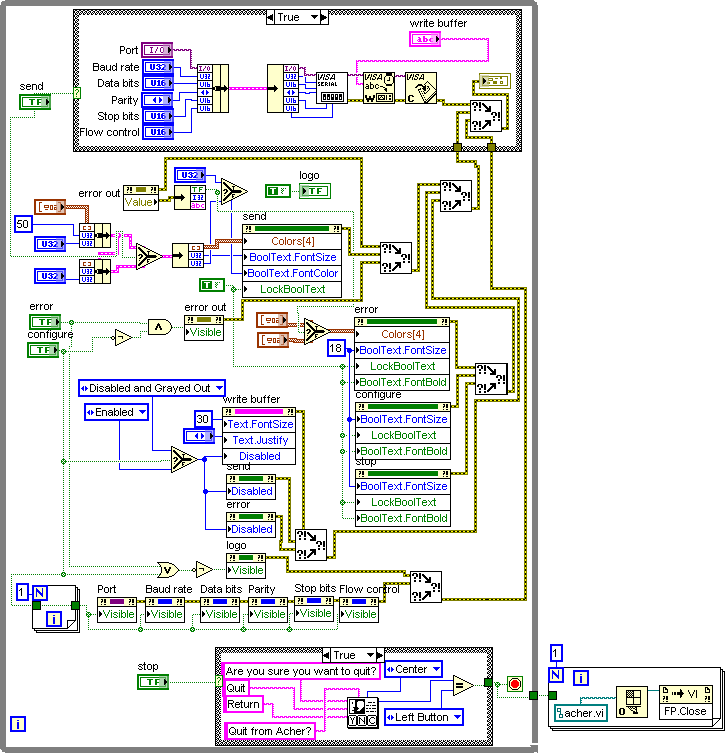
\includegraphics[width=400pt]{./images/acher_labview.png}

%--------------------------------------------------------------------------

\newpage
\begin{center}
 \textcolor{White}{.} \\
 \vspace{9cm}
 \section*{\Huge{\textbf{\underline{Anexo B}}}}\label{anexob}
\end{center}

\newpage
  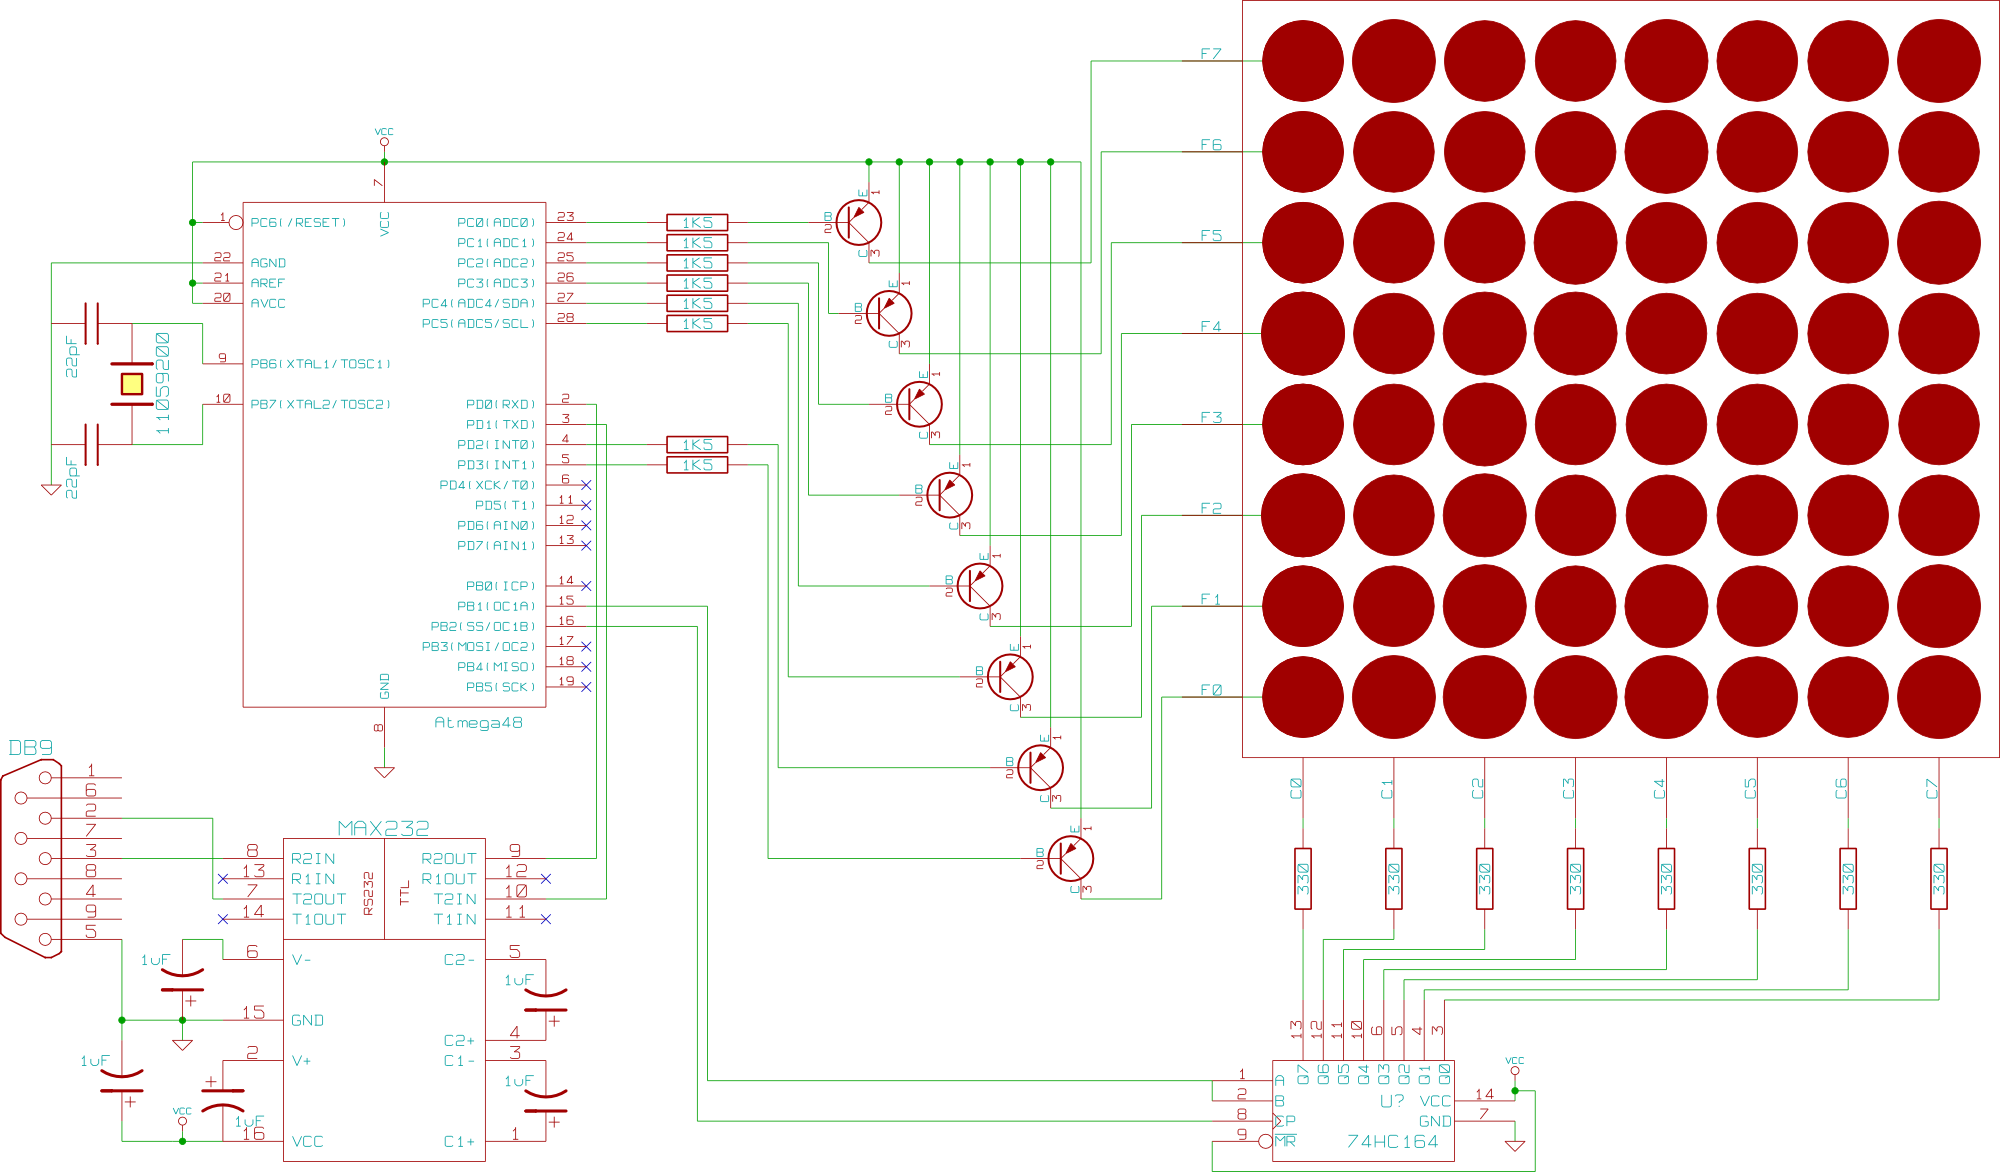
\includegraphics[angle=90,width=400pt]{./images/esq.png}

%--------------------------------------------------------------------------

\newpage
\begin{center}
 \textcolor{White}{.} \\
 \vspace{9cm}
 \section*{\Huge{\textbf{\underline{Anexo C}}}}\label{anexoc}
\end{center}

\newpage
  \textcolor{White}{.} \\
  \vspace{1.5cm} \\
  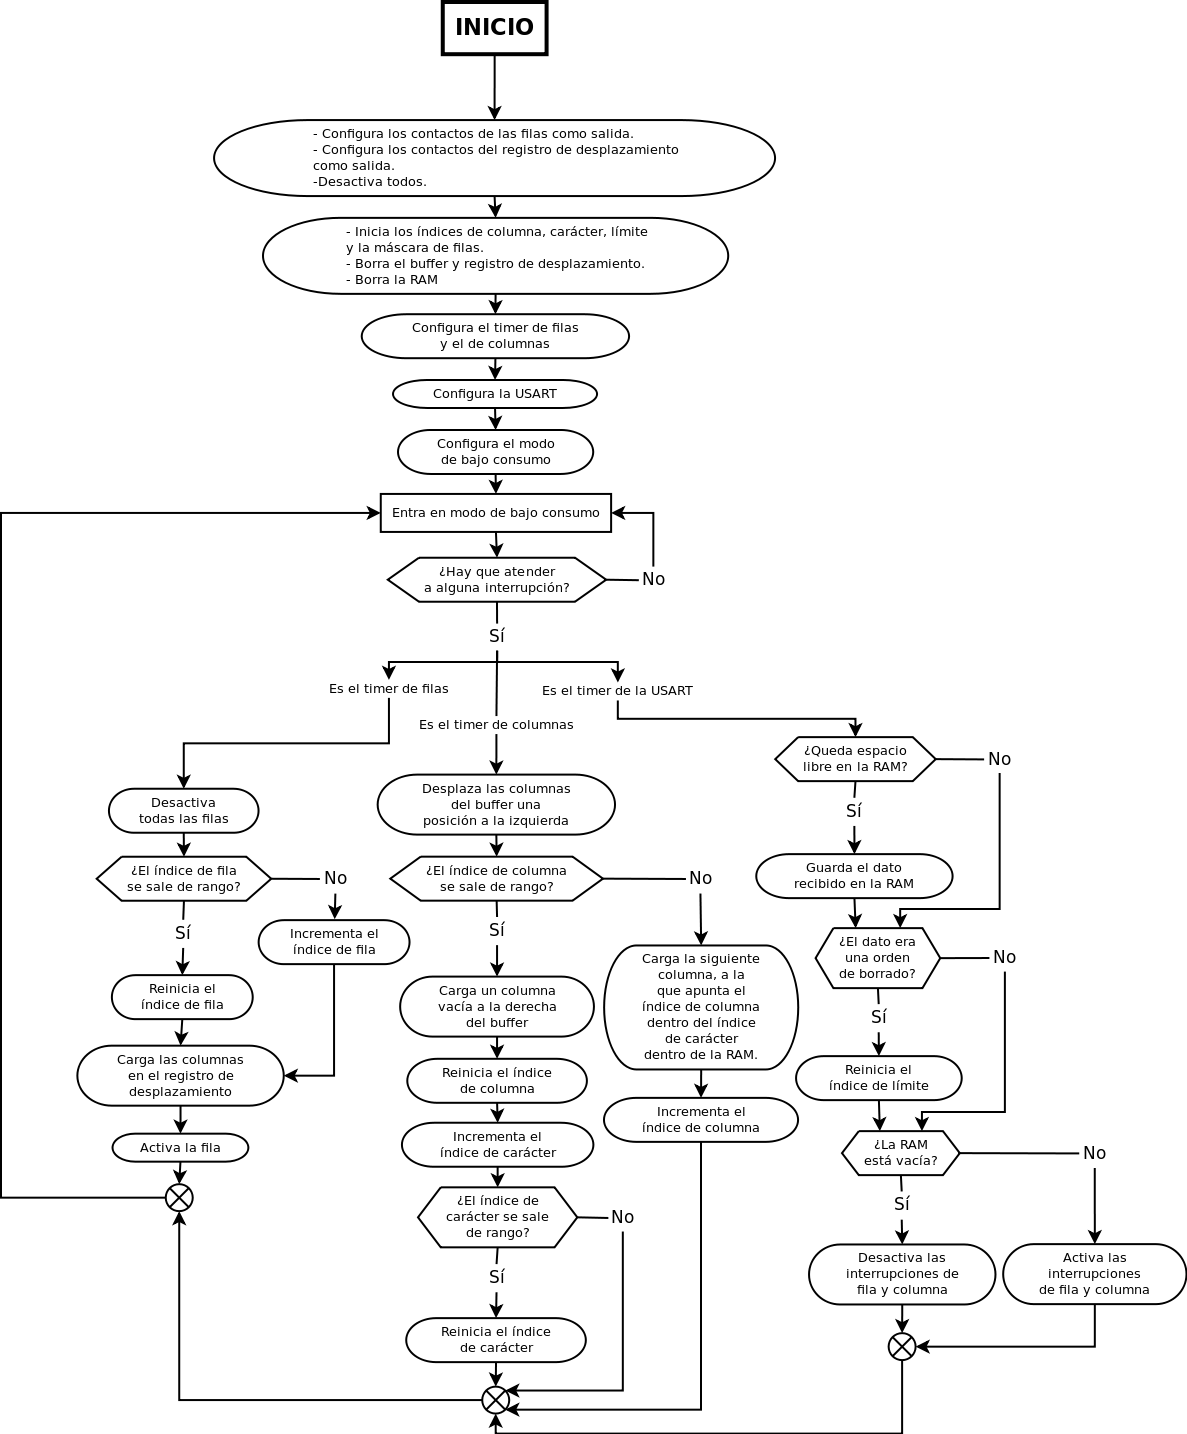
\includegraphics[width=425pt]{./images/dia_flujo.png}

\end{document}
